% $File: report.tex
% $Date: Tue Jan 06 19:48:44 2015 +0800
% $Author: jiakai <jia.kai66@gmail.com>

\documentclass[a4paper]{article}
\usepackage{amsmath,amssymb,amsthm,fontspec,verbatim,graphicx,subcaption,dirtree}
\usepackage[hyperfootnotes=false,colorlinks,linkcolor=black,anchorcolor=black,citecolor=black]{hyperref}
\usepackage[top=2in, bottom=1.5in, left=1in, right=1in]{geometry}
 
\newcommand{\addplot}[1]{\begin{center}
	\includegraphics[width=0.6\paperwidth,height=0.2\paperheight,keepaspectratio]{#1}
\end{center}}

% minted
% \inputmintedConfigured[additional minted options]{lang}{file path}
\usepackage{minted}
\newcommand{\inputmintedConfigured}[3][]{\inputminted[fontsize=\scriptsize,
	label=#3,linenos,frame=lines,framesep=0.8em,tabsize=4,#1]{#2}{#3}}
% \*src[additional minted options]{file path}
\newcommand{\cppsrc}[2][]{\inputmintedConfigured[#1]{cpp}{#2}}

% bib 
\usepackage{biblatex}
\bibliography{refs.bib}
\defbibheading{bibliography}{\section{参考文献}}

% math
\usepackage{bm}
\newcommand{\trans}[1]{#1^\intercal}
\numberwithin{equation}{section}
\renewcommand{\vec}[1]{\boldsymbol{#1}}
\newcommand{\dif}{\mathrm{d}}
\usepackage{mathtools}
\DeclarePairedDelimiter{\ceil}{\lceil}{\rceil}
\DeclareMathOperator*{\argmin}{arg\,min}

% \textref{marker}{text}
\newcommand{\textref}[2]{\hyperref[#1]{#2}}
\newcommand{\figref}[1]{\hyperref[fig:#1]{\figurename~\ref*{fig:#1}}}
\newcommand{\eqnref}[1]{\hyperref[eqn:#1]{(\ref*{eqn:#1})}}
\newcommand{\secref}[1]{\hyperref[sec:#1]{\ref*{sec:#1}节}}

% zhspacing
\usepackage{zhspacing}
\zhspacing

\newlength{\figwidth}
\setlength{\figwidth}{150mm}

\renewcommand{\today}{\number\year 年 \number\month 月 \number\day 日}
\renewcommand{\abstractname}{摘要}
\renewcommand{\contentsname}{目录}
\renewcommand{\tablename}{表}
\renewcommand{\figurename}{图}

\title{Hearv: 基于卷帘快门相机视频中物体震动的声音信号被动恢复}
\author{清华大学\\贾开~宋方睿}
\date{}

\begin{document}
\maketitle
\begin{abstract}
    声音会造成物体表面的震动。Davis等人在\cite{Davis2014VisualMic}
    中描述了通过在高速摄影的视频里分析物体表面震动来恢复环境声音的方法,
    并且也对在没有高速摄影的情况下通过卷帘快门相机视频来分析物体运动的
    方法进行了简单介绍。在本文中,我们着重研究后者的具体方法,
    并且在相对简陋的实验条件下成功恢复出了10倍于视频帧率的信号。
\end{abstract}
\tableofcontents
% $File: intro.tex
% $Date: Wed Jan 07 20:32:05 2015 +0800
% $Author: jiakai <jia.kai66@gmail.com>

\section{引言}
声音的本质是震动,人的听觉也是由于空气带动鼓膜震动进而引发一系列神经反应
而形成的。声波在媒介中传播,当它碰到物体后,会使物体表面产生微小震动。
取决于各种条件,物体表面可能会跟随环绕的媒介一起移动或者因它的震动模式变形。
在这两种情况下,运动模式包含了可用于恢复声音或了解的物体结构的信息。

物体因声音而导致的振动在近年来已被用于远程声音获取,
在监视和安全领域有重要的作用,如远程窃听谈话。
现有的采集声音的方法大多是主动的,例如需将激光束或图案投影到物体的振动表面。

Davis等人指出\cite{Davis2014VisualMic},物体振动往往能产生足够的视觉信号,
通过使用一个高速摄像机就可以部分恢复产生它们的声音。 
这一方法恢复的声音的质量不如主动方法,但是它据有一些优点,
比如不需要主动的激光照射、不需要物体具有良好的材质等。
由于在视频的每一像素观测得到了声音的空间测量,
这一方法还可以用于其他分析,比如声音导致的物体形变等。

而\cite{Davis2014VisualMic}的主要篇幅集中在基于高速摄影的全局运动恢复与
对恢复出的音频信号的后处理,对于利用卷帘快门(rolling shutter)从商用数码相机
的视频中恢复声音的技术仅进行了简单的描述。

在本文中,我们尝试在非实验室条件下,使用普通设备与商用数码相机,
从视频中基于物体表面的震动来被动地恢复拍摄视频时的环境声音。
本工作的主要贡献如下:
\begin{enumerate}
    \item 提出一种简单的卷帘快门线延迟测量方法,
        在硬件上仅需要未知频率的高频LED光源。
    \item 基于Riesz变换,辅以我们提出的朝向平滑算法,
        实现了对2D图像局部1D运动的分析并将其用于音频重建。
    \item 提出了基于多尺度频谱平均的单帧音频重建算法MSA。
    \item 提出了基于频谱指数插值和G\&L算法的全局音频重建算法。
\end{enumerate}

% vim: filetype=tex foldmethod=marker foldmarker=f{{{,f}}}



% $File: method.tex
% $Date: Wed Jan 07 23:08:41 2015 +0800
% $Author: jiakai <jia.kai66@gmail.com>

\section{方法}

在本节中介绍我们所采用的算法,分为卷帘快门、局部运动分析、单帧频谱恢复和
时域信号重建四大方面。

\subsection{卷帘快门建模及参数估计\label{sec:rolling-shutter}}
% f{{{
数码相机的快门一般有全局快门和卷帘快门两大类。对于卷帘快门,快门速度为$E$时,
其第$y$行对应的曝光时段近似为:
\begin{equation}
    I_y = [yd, yd+E]
\end{equation}
其中$d$是线延迟,也就是感光器的两行像素间曝光的时间差。这样,
如果把每行看作单独的一帧,我们相当于达到了$1/d$的采样率。

\cite{Davis2014VisualMic}采取测量直线斜率的方法得到Pentax K-01
相机的线延迟为16微秒,但没有详述其具体实现。我们缺乏生成高速运动直线的设备,
在仅有未知频率高速频闪LED的情况下实现了对线延迟的测量。

对于具有亮度调节功能的LED灯,其实现低亮度的方法往往是降低光源信号的占空比,
因此相当于有一个高速频闪的光源。在较高快门下对这样的光源录影,可得到条纹图像,
如\figref{rolling-shutter-record}所示。
\begin{figure}[h!]\begin{center}
    \begin{subfigure}[b]{.5\figwidth}
        \centering
        \includegraphics[width=.5\figwidth]{res/rolling0.png}
        \caption{1/1000s 快门速度}
    \end{subfigure}
    \begin{subfigure}[b]{.5\figwidth}
        \centering
        \includegraphics[width=.5\figwidth]{res/rolling1.png}
        \caption{1/4000s 快门速度}
    \end{subfigure}
    \caption{用卷帘快门对高速频闪光源下的坐标纸成像结果
        \label{fig:rolling-shutter-record}}
\end{center}\end{figure}

设$[T_0, T_1]$时段里光源点亮,则此时能呈现亮条的行$y$需满足条件:
\begin{equation}
    [yd, yd+E] \cap [T_0, T_1] \ge T_\theta
\end{equation}
其中$T_\theta$为需要点亮一行像素所需的最短曝光时间。如果光源点亮时长恒定,
当$E$变化时,亮条高度也会变化,有如下关系:
\begin{equation}
    \Delta_H d \approx \Delta_E
\end{equation}

因此通过测量亮条高度和快门速度间的关系,可以推出线延迟。
我们购买了与\cite{Davis2014VisualMic}中同样型号的相机,
测量七组数据求得的平均线延迟为18.3微秒,与原文中的结论较为接近,
对应的采样率约为54644Hz。
% f}}}

\subsection{运动分析:基于Complex Steerable Pyramid分解}
% f{{{
\cite{Davis2014VisualMic}采取了基于Complex Steerable Pyramid的方法进行运动恢复,
由于其实现比较复杂,效率更低,而且需要预先定义好几个离散的朝向而未被我们采用;
但在此我们也对其进行简单叙述。

Complex Steerable Pyramid是可以把图片分解为不同方向和尺度的子频带滤波器组,
最初由Portilla和Simoncelli提出用于纹理分析和合成\cite{Portilla99}。
对于单通道图像$I: \mathbb{Z}^2 \mapsto \mathbb{R}$和给定的尺度$r$及旋转方向
$\theta$,在$I$的每一个局部$(x, y)$附近,可利用Complex Steerable Pyramid
将其对应的频带表示为:
\begin{equation}
    A(r, \theta, x, y) e^{i\varphi(r, \theta, x, y)}
\end{equation}
扩展到视频中,可得到$t$时刻时某空间位置对应的相位$\varphi(r, \theta, x, y, t)$。
则相对某参考帧$t_0$的相位差
\begin{equation}
    \varphi_v(r, \theta, x, y, t) = \varphi(r, \theta, x, y, t) - 
    \varphi(r, \theta, x, y, t_0)
\end{equation}
对应于$t$时刻$(x, y)$点在$(r, \theta)$方向上的运动。

有了局部运动信息后,对每个$(r_i, \theta_i)$二元组计算全局平均运动:
\begin{equation}
    \Phi(r_i, \theta_i, t) = \sum_{x, y}
    A(r, \theta, x, y, t)^2 \varphi_v(r, \theta, x, y, t)
\end{equation}

随后,在时间上对$\Phi(r_i, \theta_i, t)$进行平移以防止不同方向的震动相抵消:
\begin{equation}
    t_i = \arg\max_{t_i} \trans{\Phi(r_0, \theta_0, t)}\Phi(r_i, \theta_i, t +
    t_i)
\end{equation}

最后,对所有$\Phi(r_i, \theta_i, t + t_i)$按$i$求平均就是$t$时刻全局运动,
对应此时的声音信号。

但该方法实现比较复杂而且计算量较大,我们目前还没测试,而是使用了下文所述的基于
Riesz变换的方法。

% f}}}

\subsection{运动分析:基于Riesz变换}
% f{{{
Riesz变换\cite{felsberg2001monogenic}是对分析信号的二维扩展。
一个一维实信号的分析信号是复信号,由原信号加上其希尔伯特变换作为虚部得到,
其具有振幅连续性,由分析信号的相位差可以检测出两个实信号的局部平移变化。
Riesz变换将此扩展到二维,可以把二维实信号分解为振幅、幅角、相位三个分量,
对于图像而言,相位变化对应原图在空域上的位移。Unser等人将此扩展到了多分辨率
\cite{unser2009multiresolution},而Wadhwa等则实现了在空域上操作的近似Riesz变换
并以此实现实时运动放大\cite{Wadhwa2014RieszPyramid}。

具体而言,Riesz变换由一对滤波器组成,其转移函数分别为
\begin{equation}
    -i\frac{\omega_x}{\parallel \overrightarrow{ \omega} \parallel},~
    -i\frac{\omega_y}{\parallel \overrightarrow{ \omega} \parallel}
\end{equation}
将其应用到子频带图像$I$上时,得到滤波器响应$(R_1, R_2)$,于是局部的振幅$A$、
主方向$\theta$和相位$\phi$满足:
\begin{equation}
    I = A\cos(\phi),~R_1 = A\sin(\phi)\cos(\theta),~
    R_2 = A\sin(\phi)\sin(\theta)
    \label{eqn:riesz:decomp}
\end{equation}

而\cite{Wadhwa2014RieszPyramid}中,作者证明了用$[0.5,0,-0.5]$和
$\trans{[0.5,0,-0.5]}$两个空域上的卷积核就可以较好地近似Riesz变换。

但Riesz变换尚未被用于物体的整体运动分析,
在\cite{Wadhwa2014RieszPyramid}中也仅用于局部运动分析来进行运动放大。
如果要用于整体分析,有个本质性的问题是
$(A, \phi, \theta)$和$(A, -\phi, \theta + \pi)$都是\eqnref{riesz:decomp}的解,
无法唯一确定相位,也就无法简单的得到在单帧中各空间位置一致的相位差。

为了解决这个问题,我们提出了朝向平滑算法。对于图像$(A(x, y), \phi(x, y),
\theta(x, y))$,设其平滑后的图像为$(A_s(x, y), \phi_s(x, y), \theta_s(x, y))$,
需要求出$k(x, y)\in \mathbb{Z}$,满足:
\begin{eqnarray}
    |\theta(x, y) + k(x, y)\pi - \theta_0(x, y)| &\le& \frac{\pi}{2} \nonumber \\
    A_s(x, y) &=& A(x, y) \nonumber \\
    \theta_s(x, y) &=& \theta(x, y) + k(x, y)\pi \nonumber \\
    \phi_s(x, y) &=& (-1)^k\phi(x, y)
\end{eqnarray}
其中$\theta_0(x, y)$为目标朝向,先各行独立进行指数滤波平滑,
$\theta_0(x+1, y) = \alpha\theta_0(x, y) + (1-\alpha)\theta_s(x, y)$,
再同理在各行之间进行平滑。平滑算法的效果如\figref{smooth}所示。
\begin{figure}[h!]\begin{center}
    \begin{subfigure}[b]{.5\figwidth}
        \centering
        \includegraphics[width=.5\figwidth]{res/smooth-0.png}
        \caption{未进行朝向平滑}
    \end{subfigure}
    \begin{subfigure}[b]{.5\figwidth}
        \centering
        \includegraphics[width=.5\figwidth]{res/smooth-1.png}
        \caption{进行朝向平滑}
    \end{subfigure}
    \caption{朝向平滑算法效果\label{fig:smooth}}
\end{center}\end{figure}

对于两帧$F_1 = (A_1, \phi_1, \theta_1)$和$F_2 = (A_2, \phi_2, \theta_2)$,
先将$F_1$按上述方法进行朝向平滑得到$F_{1s}$,再令上述算法中的
$\theta_0=\theta_{1s}$对$F_2$平滑得到$F_{2s}$,使得$\theta_{2s}$与$\theta_{1s}$
尽量接近,于是可得全局相位差
\begin{equation}
    \delta_\phi(F_1, F_2) = \sum_{x, y}
    \left(\frac{A_{1s}(x, y) + A_{2s}(x, y)}{2}\right)^2(\phi_{2s}(x, y) -
    \phi_{1s}(x, y))
    \label{eqn:global-phasediff}
\end{equation}

另外,在基于视频进行运动恢复的情况下,
我们也尝试了其它的消除$(\phi, \theta)$和$(-\phi, \theta+\pi)$歧义的方法。
取二元组$Q=(\phi\sin(\theta), \phi\cos(\theta))$,则$Q$是不存在这种歧义的,
但每个点的运动信号都变成了二维。于是对每个点,可取出其在各帧的$Q$值,
进行主分量分析(PCA)投影到一维,得到该点的一维运动信号。
但实验发现这种方法效果并不好。

% f}}}

\subsection{单帧卷帘快门图像中的高频信号分析:MSA算法\label{sec:algo-hf}}
% f{{{
使用前述Complex Steerable Pyramid分解或者在Laplacian Pyramid
的每一级使用上述Riesz变换,均可得到图像在某个尺度下局部的运动情况。
下一步的问题就是如何利用该信息和前述的卷帘快门性质,来恢复曝光时间段内的信号。

具体而言,现在已知$(A_\theta(x, y), D_\theta(x, y))$,
分别为在$\theta$的尺度下,当前帧和参考帧在$(x, y)$处的振幅均值和相位差。
其中$\theta$为非负整数,表示当前尺度的空间分辨率为原图的$\frac{1}{2^\theta}$。

\cite{Davis2014VisualMic}中主要处理了对全局震动的恢复,
但对基于卷帘快门图像的具体恢复方法没有详述;在此我们借鉴了其中的一些思想,
提出了多尺度频谱平均算法,简称为MSA(Multi-scale Spectrum Averaging)。

$(A_\theta(x, y), D_\theta(x, y))$描述的是局部运动,
我们的基本思想是在同一尺度的相邻空间范围内对局部运动加权平均,
再对得到的平均运动进行DFT变换得到频谱,最后将各频谱在对应频率上的功率进行平均,
最终的到这段时间内原始信号的功率谱。这样做主要出于以下两点原因:
\begin{enumerate}
    \item 物体表面的震动分布很复杂,如果简单的进行全局的运动平均,
        很可能各部分的震动由于相位差而相互抵消,导致平均信号中信息丢失;
    \item 人耳主要对各频率的能量敏感而对相位不敏感,
        这样我们可以对频谱的功率进行平均,
        并仍能保证重建出的信号与原信号相比对人耳的区别不大
        \footnote{这方面没找到权威文献,可参考
            \url{http://en.wikipedia.org/wiki/Audio\_system\_measurements}
        中的Phase distortion部分}。
\end{enumerate}

具体而言,对于$\theta$尺度,设图像大小为$H_\theta \times W_\theta$;
另外需要先确定参数$g_\theta$,表示按列进行分组平均的组的大小。
随后用振幅加权得到各组的时域信号、功率谱及权重:
\begin{eqnarray}
    x_\theta^i(t) &=& \frac{\sum_{k=ig_\theta}^{(i+1)g_\theta-1}
    A_\theta(k, t)D_\theta(k, t)}
        {\sum_{k=ig_\theta}^{(i+1)g_\theta-1}A_\theta(k, t)} \\
    X_\theta^i(\omega) &=& |\text{DFT}(x_\theta^i)(\omega)| \\
    w_\theta^i &=& \sum_{t=1}^{H_\theta}
        {\sum_{k=ig_\theta}^{(i+1)g_\theta-1}A_\theta(k, t)} \\
    && \text{其中,} 0 \le i \le \frac{W_\theta}{g_\theta} - 1 \nonumber
\end{eqnarray}

需要注意的是$(W_\theta, H_\theta) = 2(W_{\theta+1}, H_{\theta+1})$,
即$X_\theta^i$的长度是$X_{\theta+1}^i$的2倍;但它们对应于原图上不同的空间尺度,
在卷帘快门下即对应于不同的采样率,因此对于合法的$\omega$,
$X_\theta^i(\omega)$和$X_{\theta+1}^i(\omega)$所实际对应的频率相同,
所以只需要把$X_\theta^i$中高频的部分丢弃即可。设取了$[0, \theta_m]$间的尺度,
则最终的平均功率谱为:
\begin{eqnarray}
    A(\omega) &=& \frac{\sum_{\theta=0}^{\theta_m}
    \sum_{i=0}^{\frac{W_\theta}{g_\theta} - 1}X_\theta^i(\omega)w_\theta^i}
    {\sum_{\theta=0}^{\theta_m}
    \sum_{i=0}^{\frac{W_\theta}{g_\theta} - 1}w_\theta^i} \\
    && \text{其中,} 0 \le \omega \le \frac{1}{2}H_{\theta_m} \nonumber
\end{eqnarray}
用$d$表示卷帘快门的线延迟,则$A(\omega)$对应于原信号中频率为
$\frac{\omega}{H_{\theta_m}d2^{\theta_m}}$的分量的功率。
% f}}}

\subsection{时域音频信号的重建\label{sec:global-opt}}
% f{{{
基于\secref{algo-hf}的算法得到视频各帧的频谱后,还需要将其在时域上拼接起来
得到一段人耳可辨识的声音。然而,如果只是简单的对各帧频谱进行IDFT变化,
是很难得到可用的音频的,原因有以下两点:
\begin{enumerate}
    \item 相位信息已经在频谱平均过程中丢失了,无法直接进行IDFT
    \item 在视频分辨率为$1280\times 720$,线延迟$18.3\mu$s的情况下,
        每帧的采样时间为0.013s,而视频帧率为60fps,两帧间隔为0.017s,
        也就是说每帧内大概有1/3的时间没有采样,有信息丢失。
\end{enumerate}

期间我们尝试过使用随机相位、overlap-add等各种方法进行全局恢复,
但由于视频帧率为60fps,这类方法总会在两帧交接处产生一些artifact,
最终导致得到的音频中有60Hz左右的beat,对人耳的听觉感知影响严重。

后来我们发现这是学术界已经研究过的一类问题:
基于修改过的短时Fourier变换的信号重建。G\&L算法\cite{griffin1984signal}
是该领域的一个经典算法,
大致思想是定义一个重建信号的STFT到给定STFT的L2距离作为损失函数,
并证明了用一个迭代公式可以收敛到局部最优解。具体而言,
对时域信号$x(n)$,用$X_w(mS, \omega)$表示其在以$S$为步长的STFT中,
第$m$个时段内$\omega$频率所对应的功率,
则时域信号$x(n)$和给定的STFT $Y_w(mS, \omega)$间的距离定义为:
\begin{equation}
    D[x(n), Y_w(mS, \omega)] = \sum_{m}\frac{1}{2\pi}
    \int_{-\pi}^{\pi}\left|X_w(mS,\omega)-Y_w(mS,\omega)\right|^2
    \dif{\omega}
\end{equation}

最终所求$x(n)=\argmin_{x(n)}D[x(n), Y_w(mS, \omega)]$,
对此,可以用下式进行迭代求解:
\begin{equation}
    x^{i+1}(n) = \frac{\sum_{m}w(mS-n)\frac{1}{2\pi}
        \int_{-\pi}^{\pi}|Y_w(mS,\omega)|\frac{
        X_w^i(mS,\omega)}{|X_w^i(mS,\omega)|}}{
        \sum_m w^2(mS-n)}
    \label{eqn:gliter}
\end{equation}
其中$w(n)$是STFT所用的窗函数。

直观上\eqnref{gliter}是很好理解的,每次迭代相当于用当前$x^i(n)$的相位和
$Y_w(mS, \omega)$所需要的功率组合得到$x^{i+1}(n)$。Griffin等在
\cite{griffin1984signal}中给出了更多细节,
并证明了这样的迭代最终会收敛到局部最优解。

另一个问题是,我们恢复出的单帧信号之间没有交叠,
不能直接用于STFT目标来进行音频恢复。对此我们的解决方法是对功率谱进行指数插值。

具体而言,对于$n$帧的视频,各帧的时间点为$t_0,\cdots t_{n-1}$,
其中$t_i=if_s^{-1}$,$f_s$是视频的帧率。另外,
记$\hat{t}=Hd$为单帧内采样的时间,其中$H$为视频图像高度,$d$为卷帘快门的线延迟。
在第$i$帧,即$[t_i, t_i+\hat{t}]$时段内恢复出的功率谱为$A_i(\omega)$。

我们以$\hat{t}$作为STFT的窗口大小,并按照\cite{griffin1984signal}中取
$S=\frac{1}{4}\hat{t}$作为STFT的步长,则STFT所需求的时间点为$t'_i=iS$。
为了得到在$t'_i$时对应的功率谱$Y_i$,先找到$j$满足$t_j\le t'_i < t_{j+1}$,取:
\begin{eqnarray}
    Y_i(\omega) &=& \exp{L(\log{A_j(\omega)}, \log{A_{j+1}(\omega)},
    \frac{t'_i-t_j}{t_{j+1}-t_j})} \\
    \text{其中, } L(p, q, \alpha) &=& (1-\alpha)p+\alpha q \nonumber
\end{eqnarray}

另外,在实现时,我们取从随机相位重建出的信号作为G\&L算法的迭代初解,
以期初始解比较平滑。

% f}}}

% vim: filetype=tex foldmethod=marker foldmarker=f{{{,f}}} 


% $File: expr.tex
% $Date: Wed Jan 07 20:05:48 2015 +0800
% $Author: jiakai <jia.kai66@gmail.com>

\section{实验}
关于卷帘快门的参数测量已在\secref{rolling-shutter}中描述,在此不再赘述。
本节中主要介绍前述算法在合成数据和实际数据上的表现情况。

\subsection{基于合成全局快门数据的全局运动分析\label{sec:synth-global}}
% f{{{
使用如下公式合成可控位移的图像,其效果如\figref{synthesis}所示:
\begin{equation}
    f(x, y) = \sin(\omega_x (x + \delta_x)) + \sin(\omega_y y) + 
    \mathcal{N}(0, \sigma^2)
    \label{eqn:synth-global}
\end{equation}
其中$\delta_x$控制位移,$\sigma$控制噪声,$f(x, y)$被量化到$[0, 255]$间的整数。
\begin{figure}[h!]\begin{center}
    \begin{subfigure}[b]{.35\figwidth}
        \centering
        
\includegraphics[width=.35\figwidth]{res/synth0.png}
    \end{subfigure}
    \begin{subfigure}[b]{.35\figwidth}
        \centering
        \includegraphics[width=.35\figwidth]{res/synth1.png}
    \end{subfigure}
    \caption{合成数据,$\delta_x = 0.01$pxl, $\sigma = 1.35/255$}
    \label{fig:synthesis}
\end{center}\end{figure}

控制$\delta_x$取不同的值,按\eqnref{global-phasediff}得到的相位差如
\figref{synthesis:pd}所示。
\begin{figure}[h!]\begin{center}
    \includegraphics[width=.5\figwidth]{res/synth-pd.png}
    \caption{位移与相位差的关系}
    \label{fig:synthesis:pd}
\end{center}\end{figure}

总的来说,基于合成数据的实验证明了前述算法的可行性,
显示相位差与实际位移线性相关,而且对噪声比较鲁棒,
在$\sigma \le 3/255$时都比较有效,已经远低于一般设备的噪声;
但在$\sigma=0$时出现了较大波动,猜测这是由于量化时取整带来的bias造成的,
而在有噪声时可一定程度上抵消这种bias。而为何在噪声太大时由正相关变成了反相关,
我们还没有找到明确的解释。

% f}}}

\subsection{基于实际数据的全局运动分析与低频信号恢复\label{sec:data-global}}
% f{{{

把坐标纸贴在扬声器的震膜上直接拍摄,用扬声器播放10hz, 15hz, 20hz, 25hz的声音,
用Pentax K-01相机拍摄,快门速度为1/2000, iso100, F/5.6, 55mm, 视频为1280x720,
59.940fps, H.264编码。

使用上述方法估计全局运动并直接作为采样信号进行FFT,
发现对单频音和多频音均能较好恢复,
多频音的结果如\figref{real:lowfreq}所示。
\begin{figure}[h!]\begin{center}
    \begin{subfigure}[b]{.5\figwidth}
        \includegraphics[width=.5\figwidth]{res/setting.png}
        \caption{实际拍摄情况}
    \end{subfigure}
    \begin{subfigure}[b]{.5\figwidth}
        \includegraphics[width=.5\figwidth]{res/global-recon.png}
        \caption{重建结果,可见对各频率均能较好恢复;
            其中后半部分的振幅偏高是由于拍摄时误碰了实验装置造成整体位移,
            但对结果影响不大}
    \end{subfigure}
    \caption{基于全局运动分析的低频信号重建}
    \label{fig:real:lowfreq}
\end{center}\end{figure}

% f}}}

\subsection{基于合成卷帘快门数据的局部运动分析,
    及基于MSA算法的高频信号恢复\label{sec:synth-local}}
% f{{{
与\secref{synth-global}类似,我们先用合成数据的方法测试算法的可行性。
对\eqnref{synth-global}进行修改,我们使用如下方法合成一段视频,对于第$i$帧:
\begin{eqnarray}
    f(i, x, y) &=& \sin(\omega_x (x + \delta_x(i, y))) + \sin(\omega_y y) + 
    \mathcal{N}(0, \sigma^2) \\
    \delta_x(i, y) &=& A\sin(2\pi f_s(it_f+yd))
    \label{eqn:synth-local}
\end{eqnarray}
实验中,在\eqnref{synth-local}里我们取$A=0.01$表示震动造成的水平位移为$0.01$像素,
$t_f=\frac{1}{60}$为视频每帧的时长,$d=1.57e-5$为线延迟,$f_s=500$为震动频率,
另外$f(i, x, y)$量化到$[0, 255]$间的整数并加上方差为1的白噪声。
另外我们还选取了$f_s=\{500, 800\},\,A=\{0.01, 0.005\}$进行多频音的测试。
对视频前10帧用\secref{algo-hf}所述的方法进行频谱恢复,
结果如\figref{synth-local}所示,
可见在噪声存在的情况下,
该方法能较为准确的恢复卷帘快门成像所包含的高频运动信息。
\begin{figure}[h!]\begin{center}
    \begin{subfigure}[b]{.5\figwidth}
        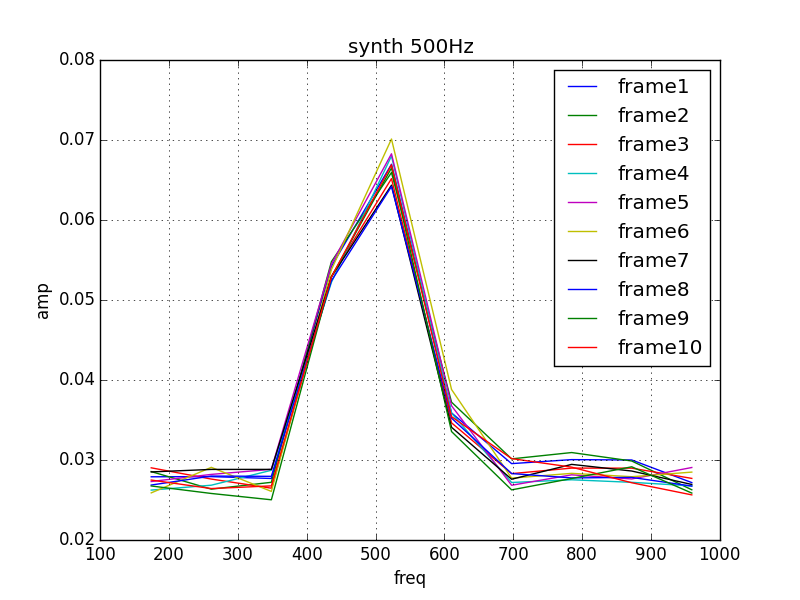
\includegraphics[width=.5\figwidth]{res/synth-500.png}
        \caption{500Hz合成数据的恢复}
    \end{subfigure}
    \begin{subfigure}[b]{.5\figwidth}
        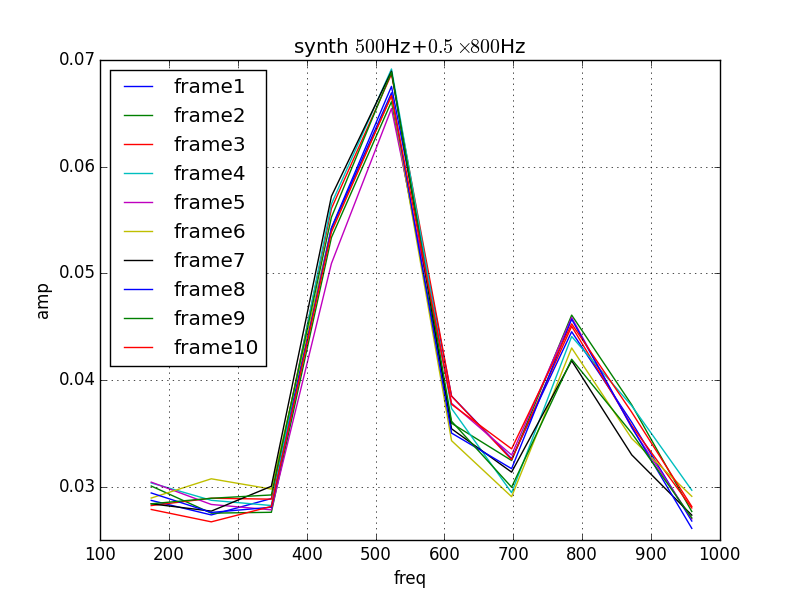
\includegraphics[width=.5\figwidth]{res/synth-500+800.png}
        \caption{500Hz和800Hz,振幅$2:1$合成数据的恢复}
        \label{fig:synth:500+800}
    \end{subfigure}
    \caption{对合成的卷帘快门视频进行频谱分析的结果}
    \label{fig:synth-local}
\end{center}\end{figure}
% f}}}

\subsection{MSA算法的合理性及其中参数的选择}
% f{{{
MSA算法中两个比较重要的参数是$\theta_m$和$g_\theta$,
分别控制图像金字塔的高度和按列分组平均的组大小。
在这里我们用实验方法确定其取值,同时也说明MSA算法的合理性。

我们采用从实际拍摄数据(见\secref{data-local})重建的频谱的信噪比
作为性能评价指标。我们已知真实数据是单频音,
因此把频谱中能量最强的频率作为信号,其余作为噪声,并随机取了
3幅参考帧和3幅目标帧,计算9次重建的平均信噪比。
调整$\theta_m$和$g_\theta$,可以得到以下数据:
\begin{figure}[h!]\begin{center}
    \begin{subfigure}[b]{.33\figwidth}
        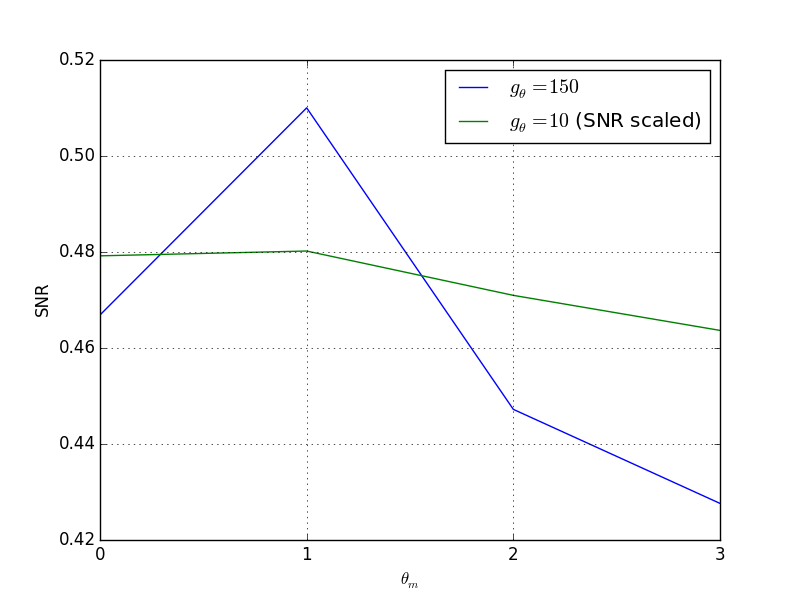
\includegraphics[width=.33\figwidth]{res/msa-lvl.png}
        \caption{SNR与$\theta_m$的关系}
        \label{fig:msa:lvl}
    \end{subfigure}
    \begin{subfigure}[b]{.33\figwidth}
        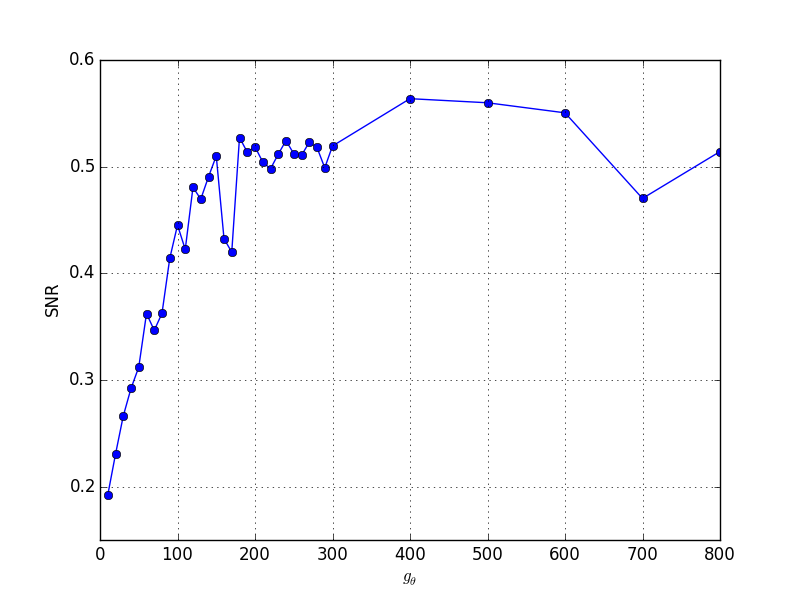
\includegraphics[width=.33\figwidth]{res/msa-vg.png}
        \caption{SNR与$g_\theta$的关系}
        \label{fig:msa:vg}
    \end{subfigure}
    \begin{subfigure}[b]{.33\figwidth}
        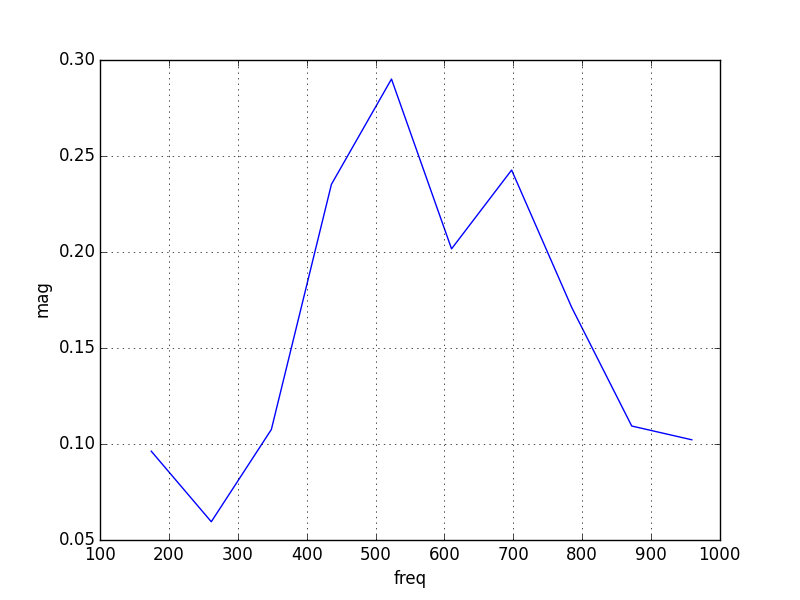
\includegraphics[width=.33\figwidth]{res/msa-800.png}
        \caption{$g_\theta$太大时的实际重建频谱}
        \label{fig:msa:800}
    \end{subfigure}
    \caption{MSA调参情况}
    \label{fig:msa}
\end{center}\end{figure}

从这些数据中有以下发现:
\begin{enumerate}
    \item \figref{msa:lvl}说明MSA中取多个尺度求平均是可以提高性能的,
        具体而言在$\theta_m=1$,即取两个尺度时性能较好;同时也说明了
        $g_\theta$和$\theta_m$对SNR的影响基本正交。
    \item 在\figref{msa:vg}中看似$g_\theta$越大越好,
        但观察在其取值较大时的实际重建频谱\figref{msa:800}可发现,
        尽管SNR比较高,却出现了两个尖峰,是很严重的artifact。
        因此一方面SNR并不是评价性能的最好指标,
        另一方面MSA中按列分组取平均也是可提高鲁棒性的。
        我们观察发现,整体而言$g_\theta$越大,
        频谱越有变宽或者出现多个尖峰的趋势,
        最终我们取了$g_\theta=150$作为比较折衷的值。
\end{enumerate}

另外,我们也尝试了对多个尺度取不同的$g_\theta$,具体而言令
$g_\theta=\frac{150}{2^\theta}$,发现SNR从0.51降至0.40,
因此最终选择了常数的$g_\theta=150$。
% f}}}

\subsection{基于实际数据和MSA算法的局部运动分析与高频信号恢复
    \label{sec:data-local}}
% f{{{
与\secref{data-global}采用相同的相机配置,如\secref{algo-hf}所述取
$\theta_m=1$,此时采样率上限为
$\frac{1}{d2^{\theta_m}} \approx 27000$Hz,
而实际可用的采样频率还受限于快门速度,大概不超过$1000$Hz。

我们对单频和双频音进行了测试,发现单频音恢复效果总体不错,
但双频音则效果很差。具体如\figref{real:highfreq}所示。
\begin{figure}[h!]\begin{center}
    \begin{subfigure}[b]{.33\figwidth}
        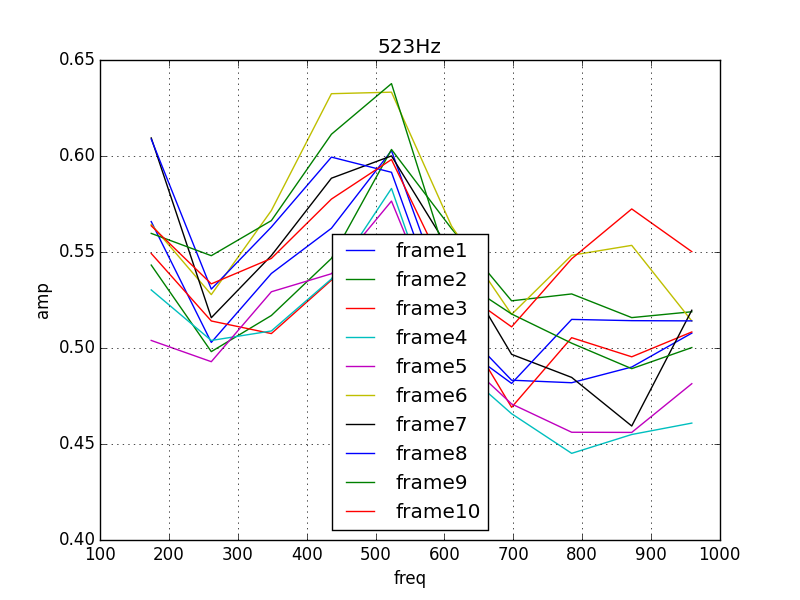
\includegraphics[width=.33\figwidth]{res/data-523.png}
        \caption{$\text{C}_5$(523Hz)单频音的恢复}
    \end{subfigure}
    \begin{subfigure}[b]{.33\figwidth}
        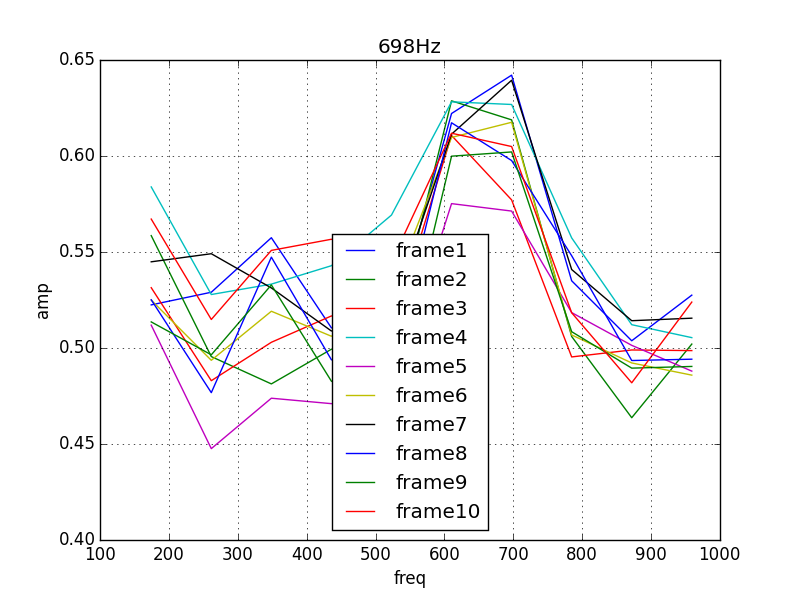
\includegraphics[width=.33\figwidth]{res/data-698.png}
        \caption{$\text{F}_5$(698Hz)单频音的恢复}
    \end{subfigure}
    \begin{subfigure}[b]{.33\figwidth}
        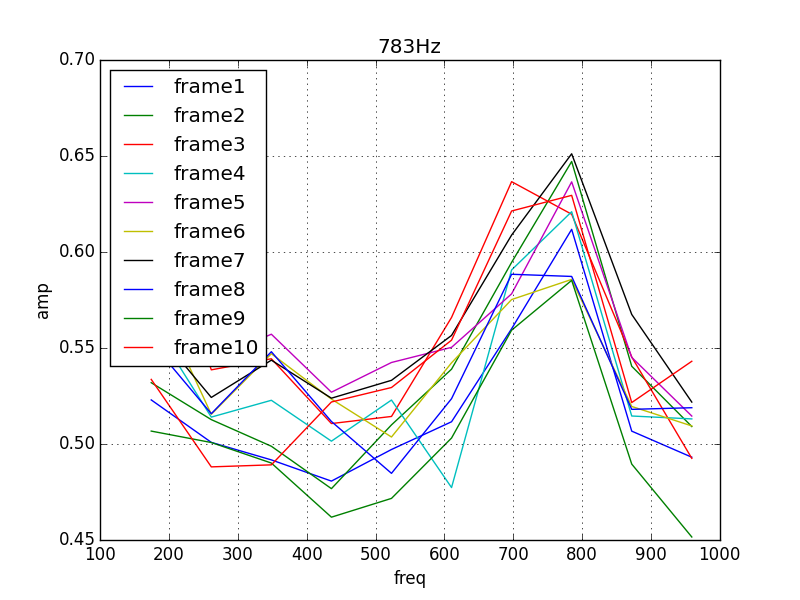
\includegraphics[width=.33\figwidth]{res/data-783.png}
        \caption{$\text{G}_5$(783Hz)单频音的恢复}
    \end{subfigure}
    \begin{subfigure}[b]{.4\figwidth}
        \includegraphics[width=.4\figwidth]{res/data-300+500.png}
        \caption{等幅300Hz+500Hz双频音的恢复}
        \label{fig:real:300+500}
    \end{subfigure}
    \begin{subfigure}[b]{.4\figwidth}
        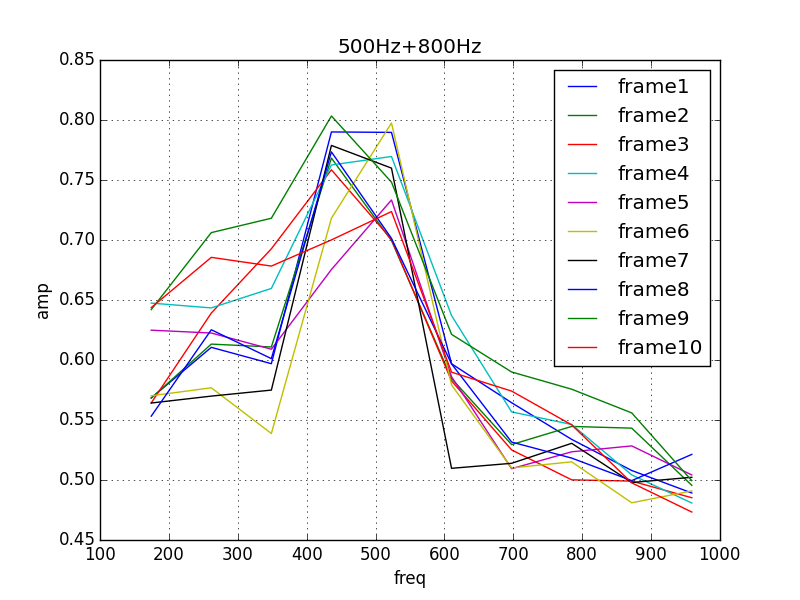
\includegraphics[width=.4\figwidth]{res/data-500+800.png}
        \caption{等幅500Hz+800Hz双频音的恢复}
    \end{subfigure}
    \caption{对实际拍摄视频进行频谱分析的结果}
    \label{fig:real:highfreq}
\end{center}\end{figure}
% f}}}

\subsection{全局优化}
% f{{{
全局优化分为频谱的指数插值和G\&L迭代两步,已在\secref{global-opt}中详述。
在这里我们展示优化过程中信号的变化情况,如\figref{global-opt}所示。
可以观察到随着迭代的进行,信号逐渐变得平滑。在大约200次迭代后,
就能得到比较稳定的解,播放后人耳可以辨认出单频音的音高。
相关视频和音频在本文的补充材料中。
\begin{figure}[h!]\begin{center}
    \begin{subfigure}[b]{\figwidth}
        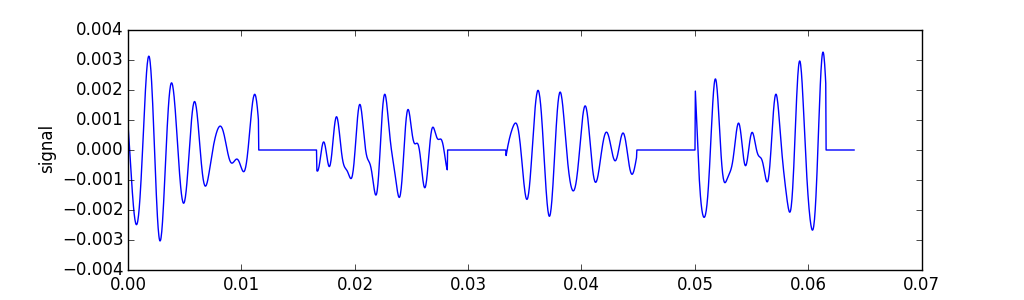
\includegraphics[width=\figwidth]{res/opt00.png}
        \caption{全局优化的初始解}
    \end{subfigure}
    \begin{subfigure}[b]{\figwidth}
        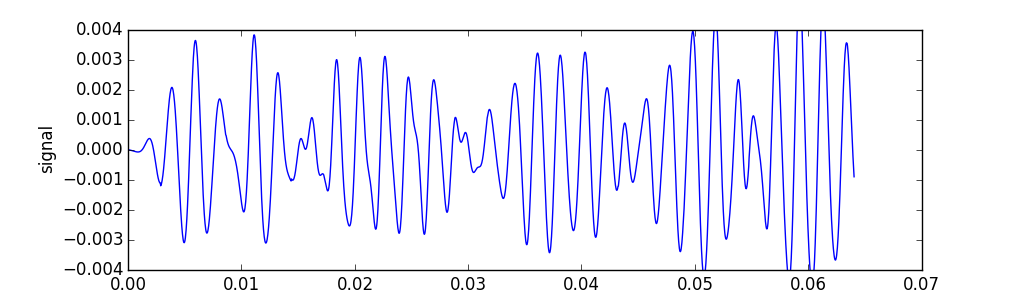
\includegraphics[width=\figwidth]{res/opt01.png}
        \caption{迭代1步后的情况}
    \end{subfigure}
    \begin{subfigure}[b]{\figwidth}
        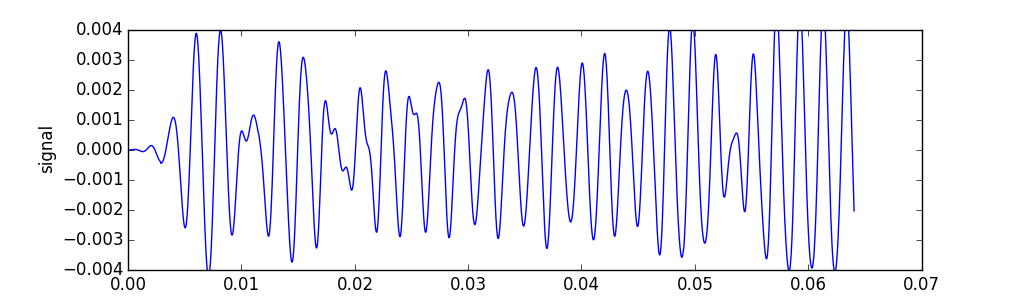
\includegraphics[width=\figwidth]{res/opt20.png}
        \caption{迭代20步后的情况}
    \end{subfigure}
    \begin{subfigure}[b]{\figwidth}
        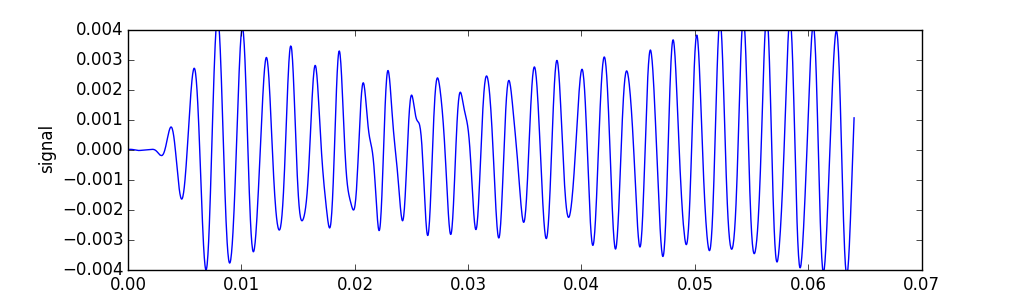
\includegraphics[width=\figwidth]{res/opt200.png}
        \caption{迭代200步后的情况}
    \end{subfigure}
    \caption{全局优化过程}
    \label{fig:global-opt}
\end{center}\end{figure}
% f}}}

% vim: filetype=tex foldmethod=marker foldmarker=f{{{,f}}} 

% $File: discuss.tex
% $Date: Sun Dec 14 00:33:39 2014 +0800
% $Author: jiakai <jia.kai66@gmail.com>

\section{分析与讨论}
通过在合成数据上的实验(\secref{synth-global}、\secref{synth-local}),
可以发现在理想情况下,
基于Riesz变换的局部运动分析的方法在恢复低频全局运动和高频逐行局部运动上
均是比较有效的,在噪声存在的情况下对于$0.01$像素的运动仍能给出明确响应。

在实际拍摄的视频上,我们发现对单频音仍能较有效的恢复。然而,
经过多次尝试,仍不能取得满意的双频音恢复效果,
也仅仅是能在\figref{real:300+500}中在500Hz附近看到一个小尖峰。
对此我们尚不能给出一个很好的解释,猜想是对实际信号中振幅相对大小恢复的不够好,
导致低频信号盖过高频信号。对比\figref{synth:500+800}的结果,
也说明我们合成的数据相对实际数据而言还是太过于理想了。

在此,先提出本工作的一些{\bf 局限性}:
\begin{enumerate}
    \item 单帧内频谱分析所对应的时域信号总时长只有$Hd \approx 0.01$s,
        因此频谱的谱线间距约为$100$Hz,频谱解析度较差。
    \item 对高频信号的恢复丢失了相位信息,虽然对音频的听觉效果影响不大,
        但毕竟有信息损失。
    \item 对于多频音尚无法有效恢复。
    \item 在音源音量较小,也就是震动不明显时,几乎无法恢复出有用的信息;
        而且即使被摄物体完全静止,也会较大噪声。这噪声来自多方面,
        但主要应该是低端相机本身的系统噪声和H.264视频编码引入的artifact。
\end{enumerate}

{\bf 下一步}工作是重建声音信号。在不考虑目前仅能有效恢复单频音的情况下,
希望利用频谱上的全部信息(而非直接取最大能量的频率作为重建结果)。
对此已进行了不少尝试,主要的困难有两个:
(1) 卷帘快门的总曝光时间少于帧时长,导致部分时间段内没有采样;
(2) 各帧的能量不统一,恢复出来的声音不平滑,听起来有强烈的低频节奏
而很难听到高频的原始信号。
接下来需要在降噪和全局平滑上进行更多努力,具体细节在以后的报告中详述。

与已有工作相比,本工作的{\bf 创新点}主要如下:
\begin{enumerate}
    \item 仅利用频率未知的高频闪烁LED光源观察到卷帘快门的效果,
        并估算出线延迟。
    \item 利用Riesz变换进行全局和局部的运动分析,并提出了空间朝向平滑的算法。
        Riesz变换可以直接在空域上进行,
        其运行速度也优于Complex Steerable Pyramid。
    \item 基于信号处理的基本原理,提出了从卷帘快门图像恢复高频震动的算法,
        这在已有的工作中也并没有专门讨论过。
\end{enumerate}

\section{后续工作}
在一到两周内实现能达到人耳可接受音质的单频音简单旋律的恢复,
随后看具体情况可能在以下一种或几种方向上尝试:
\begin{enumerate}
    \item 拍摄实际物体的震动而非扬声器表面的震动,
        尝试对声音的恢复
    \item 实现Complex Steerable Pyramid并进行效果的对比
    \item 设法解决多频音恢复的问题,尝试对更复杂的声音,包括语音、音乐等的恢复
\end{enumerate}

% vim: filetype=tex foldmethod=marker foldmarker=f{{{,f}}} 


\printbibliography
\end{document}

% vim: filetype=tex foldmethod=marker foldmarker=f{{{,f}}}

